\documentclass[tikz,border=15pt]{standalone}
\usepackage{tikz}
\usepackage{amsmath}
\usetikzlibrary{arrows.meta,positioning,shapes,fit}

\begin{document}
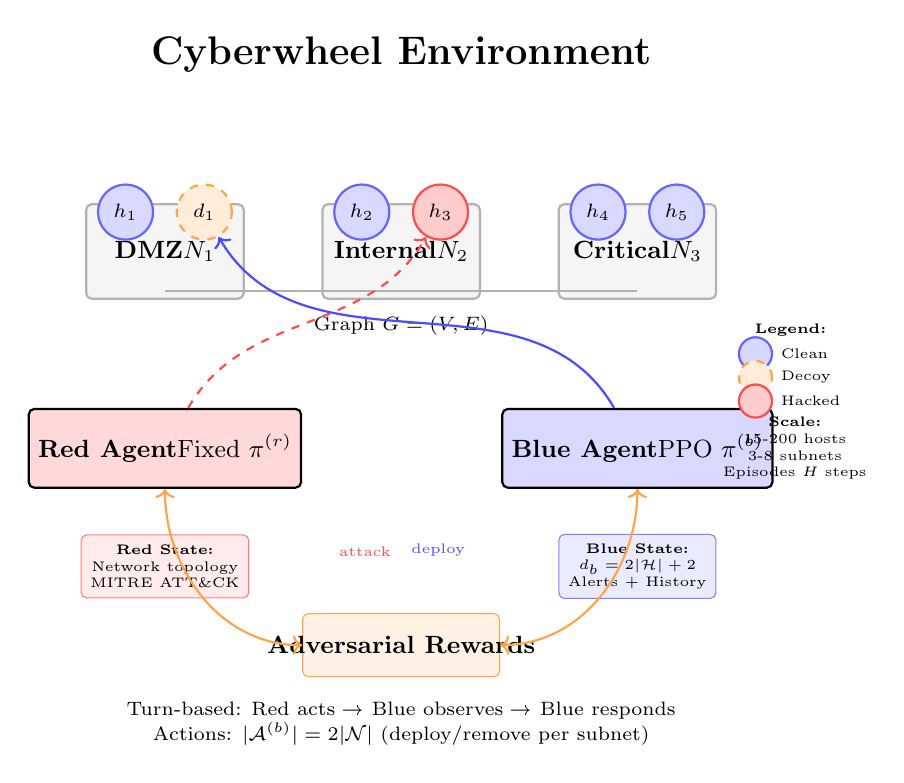
\begin{tikzpicture}[
    % Clean, minimal styles
    host/.style={circle, draw=blue!60, fill=blue!15, minimum size=7mm, font=\scriptsize, thick},
    decoy/.style={circle, draw=orange!70, fill=orange!15, minimum size=7mm, font=\scriptsize, thick, dashed},
    compromised/.style={circle, draw=red!70, fill=red!20, minimum size=7mm, font=\scriptsize, thick},
    subnet/.style={rectangle, draw=gray!60, fill=gray!8, minimum width=20mm, minimum height=12mm, font=\small, thick, rounded corners=2pt},
    agent/.style={rectangle, draw=black, fill=yellow!15, minimum width=20mm, minimum height=10mm, font=\small, thick, rounded corners=2pt},
    infobox/.style={rectangle, draw=gray!50, fill=gray!5, rounded corners=2pt, font=\tiny, align=center, minimum width=18mm, minimum height=8mm},
    node distance=4cm
]

% Title - simple and clean
\node[font=\Large\bfseries] at (0, 6.5) {Cyberwheel Environment};

% Network layer - well-spaced subnets
\node[subnet] (subnet1) at (-3, 4) {\textbf{DMZ}\\$N_1$};
\node[subnet] (subnet2) at (0, 4) {\textbf{Internal}\\$N_2$};  
\node[subnet] (subnet3) at (3, 4) {\textbf{Critical}\\$N_3$};

% Key hosts - minimal but representative
\node[host] (h1) at (-3.5, 4.5) {$h_1$};
\node[decoy] (d1) at (-2.5, 4.5) {$d_1$};

\node[host] (h2) at (-0.5, 4.5) {$h_2$};
\node[compromised] (h3) at (0.5, 4.5) {$h_3$};

\node[host] (h4) at (2.5, 4.5) {$h_4$};
\node[host] (h5) at (3.5, 4.5) {$h_5$};

% Network backbone - clean connection
\draw[thick, gray!60] (-3, 3.5) -- (0, 3.5) -- (3, 3.5);
\node[below, font=\scriptsize] at (0, 3.3) {Graph $G = (V,E)$};

% Agents - well separated
\node[agent, fill=red!15] (red) at (-3, 1.5) {\textbf{Red Agent}\\Fixed $\pi^{(r)}$};
\node[agent, fill=blue!15] (blue) at (3, 1.5) {\textbf{Blue Agent}\\PPO $\pi^{(b)}$};

% Key interactions - minimal arrows
\draw[->, thick, red!70, dashed] (red) to[out=60, in=240] (h3) node[midway, above left, font=\tiny] {attack};
\draw[->, thick, blue!70] (blue) to[out=120, in=300] (d1) node[midway, above right, font=\tiny] {deploy};

% Essential information boxes - well spaced
\node[infobox, draw=blue!50, fill=blue!8] (blue_info) at (3, 0) {
    \textbf{Blue State:}\\
    $d_b = 2|\mathcal{H}| + 2$\\
    Alerts + History
};

\node[infobox, draw=red!50, fill=red!8] (red_info) at (-3, 0) {
    \textbf{Red State:}\\
    Network topology\\
    MITRE ATT\&CK
};

% Reward system - centered and clean
\node[rectangle, draw=orange!70, fill=orange!10, minimum width=25mm, minimum height=8mm, rounded corners=2pt] (reward) at (0, -1) {};
\node[font=\small] at (reward.center) {\textbf{Adversarial Rewards}};

% Clean reward connections
\draw[<->, orange!70, thick] (red) to[out=270, in=180] (reward);
\draw[<->, orange!70, thick] (blue) to[out=270, in=0] (reward);

% Key mathematical info - bottom
\node[font=\scriptsize, align=center] at (0, -2) {
    Turn-based: Red acts → Blue observes → Blue responds\\
    Actions: $|\mathcal{A}^{(b)}| = 2|\mathcal{N}|$ (deploy/remove per subnet)
};

% Minimal legend - corner  
\node[font=\tiny, align=left] at (5, 3) {
    \textbf{Legend:}
};
\node[host, scale=0.6] at (4.5, 2.7) {};
\node[right, font=\tiny] at (4.7, 2.7) {Clean};
\node[decoy, scale=0.6] at (4.5, 2.4) {};
\node[right, font=\tiny] at (4.7, 2.4) {Decoy};
\node[compromised, scale=0.6] at (4.5, 2.1) {};
\node[right, font=\tiny] at (4.7, 2.1) {Hacked};

% Environment stats - corner
\node[font=\tiny, align=center] at (5, 1.5) {
    \textbf{Scale:}\\
    15-200 hosts\\
    3-8 subnets\\
    Episodes $H$ steps
};

\end{tikzpicture}
\end{document>